\documentclass[10pt]{article} % dà errore perchè non trova citazioni, ignorabile perchè compila comunque
\usepackage[utf8]{inputenc}
\usepackage{listings}
\usepackage{xcolor}
\usepackage{subcaption}
\usepackage{longtable}
\usepackage{booktabs}
\usepackage{enumitem}
\usepackage{hyperref}

\hypersetup{
	colorlinks,
	citecolor=black,
	filecolor=black,
	linkcolor=black,
	urlcolor=black
}

\definecolor{codegreen}{rgb}{0,0.6,0}
\definecolor{codegray}{rgb}{0.5,0.5,0.5}
\definecolor{codepurple}{rgb}{0.58,0,0.82}
\definecolor{backcolour}{rgb}{0.95,0.95,0.92}
\usepackage{color}   %May be necessary if you want to color links
\usepackage{hyperref}
\usepackage{graphicx}
\usepackage{adjustbox}
\graphicspath{ {./images/} }
\hypersetup{
    colorlinks=true, %set true if you want colored links
    linktoc=all,     %set to all if you want both sections and subsections linked
    linkcolor=black,  %choose some color if you want links to stand out
    urlcolor=blue,
}
\lstdefinestyle{mystyle}{
    backgroundcolor=\color{backcolour},   
    commentstyle=\color{codegreen},
    keywordstyle=\color{magenta},
    numberstyle=\tiny\color{codegray},
    stringstyle=\color{codepurple},
    basicstyle=\ttfamily\footnotesize,
    breakatwhitespace=false,         
    breaklines=true,                 
    captionpos=b,                    
    keepspaces=true,                 
    numbers=left,                    
    numbersep=5pt,                  
    showspaces=false,                
    showstringspaces=false,
    showtabs=false,                  
    tabsize=2
}

\lstset{style=mystyle}

\bibliographystyle{plain}

\title{DD}
\author{Mauro Famà, Giacomo Lombardo}
%\date{October 2021}

\begin{document}
\thispagestyle{empty}
\begin{titlepage}
    \newcommand{\HRule}{\rule{\linewidth}{0.5mm}}
    \center
    
\includegraphics[width=8cm]{polimi.png}\\[1cm]

    \textsc{\Large Software Engineering II}\\[0.5cm]
    \textsc{\large A.Y. 2021/22}\\[0.5cm]

    \HRule \\[0.4cm]
        { \Huge \bfseries DREAM}\\[0.2cm]
        { \large Data-dRiven prEdictive fArMing}\\[0.4cm]
        { \LARGE Design Document}
    \HRule \\[1.5cm]

    \begin{minipage}{0.4\textwidth}
        \begin{flushleft} \large
        \emph{Authors:}\\
        Mauro \textsc{Famà}\\
        Giacomo \textsc{Lombardo}\\
        \end{flushleft}
    \end{minipage}\\[2cm]

    {\large January 9, 2022}\\[2cm]
    
    \vfill
\end{titlepage}
\newpage
\tableofcontents %this command creates an index
\newpage
\section{Introduction}
\subsection{Purpose}
The purpose of this document is to comprehensively describe the design of the DREAM platform. %(reference to rasd or assignment)
It will be described the architecture of the system and its characteristics, 
moreover will be analyzed its components explaining their functionalities.\\
This document was written following the RASD of the same project, 
in fact the assumptions and design choices are based on the assumptions already explained, 
however maintaining independence between the documents. This document focuses on the explanation 
about the Software-To-Be, its modules, its interfaces and its implementation.
\subsection{Scope}
The main objective of the platform is to create a support tool and communication channel for farmers in Telangana, 
leveraging the IT infrastructure of government resources. The platform also aims to be a 
supervisory and control system for the authorities of the Ministry of Agriculture in Telangana, 
providing accurate and bulk data of farmers' performance, reducing the overhead due to manual retrieval of this information.\\
The system will have two separate and exclusive interfaces, one dedicated to PMs in Telangana 
and one dedicated to farmers in the region. Farmers will be provided with a browser 
executable web application, it will provide a dashboard to monitor the sensors embedded 
in their fields, weather forecasts for the local area and summarize the resources 
obtained and consumed by the plantations. In addition to the monitoring functionality, 
from the farmer's dashboard it will be possible to compile reports to be sent to the PM 
responsible for the area, combining data entered manually by the farmer, data created by 
IoT devices and data retrieved from the internet.\\
The web application also provides access to the forum dedicated to the Telangana farming community, 
connecting all participants in the DREAM program through its threads.
Farmers will also be able to submit their help requests into the system, which will be automatically forwarded 
to the PM responsible for the area, who in turn will have a dedicated dashboard exclusively for the administrative side.
From his application, the PM will be able to forward responses to help requests, monitor the performance of 
farmers in his area, all while viewing data from sensors and weather forecasts.
From his dashboard, the PM will have the tools to perform end-of-quarter performance evaluations, 
including direct communication channels to affected farmers.\\
There is no platform that currently provides these functions, in fact this document refers to the design of a system 
created from scratch, without any integration of existing systems, but exploiting the IT infrastructure 
already physically installed in the Telangana region.

\subsection{Definitions, Acronyms, Abbreviations}
\subsection{Revision History}
\subsection{Reference Documents}
\subsection{Document Structure}
\section{Architectural Design}
\subsection{Overview}
\begin{figure}[h]
    \centering
    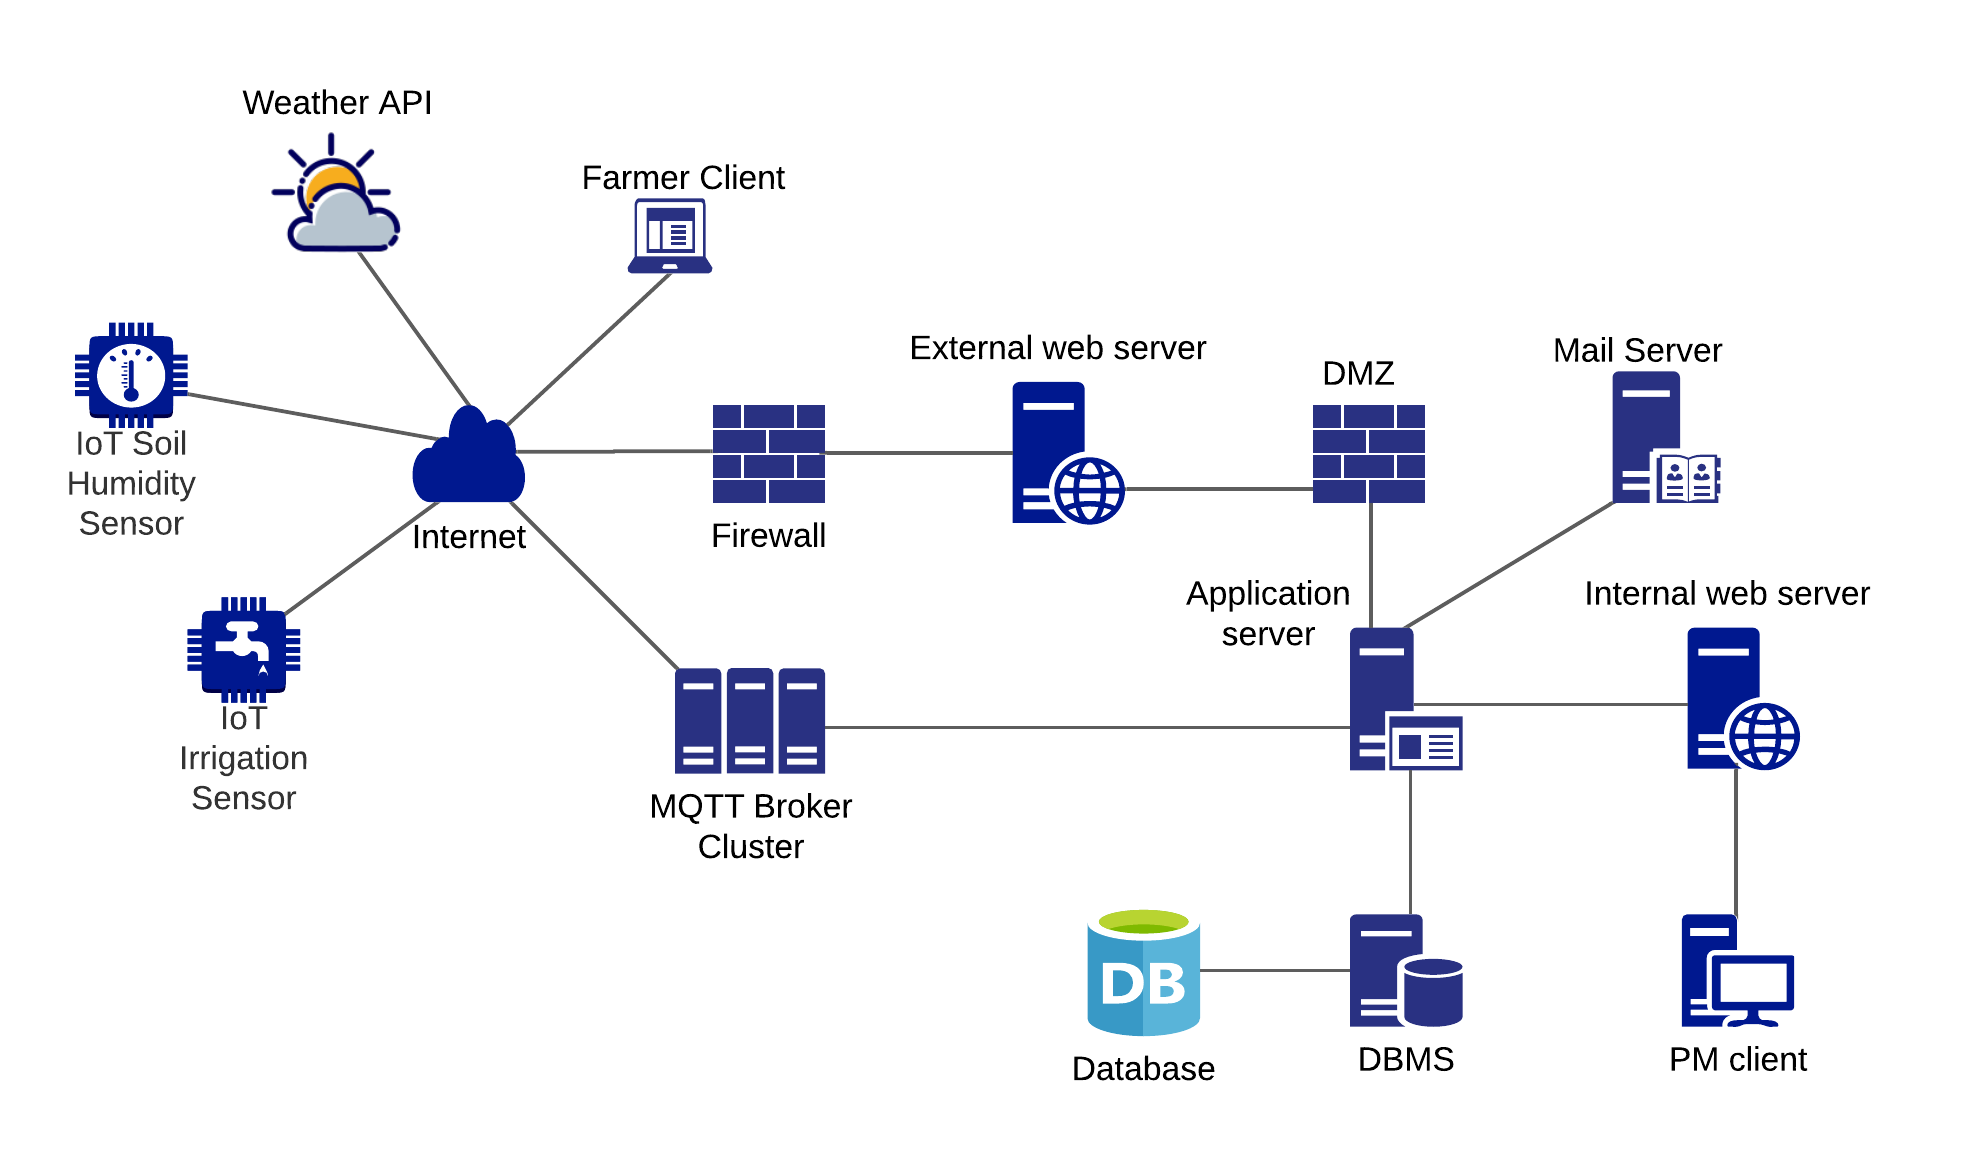
\includegraphics{images/overview_architecture.png}
    \caption{System architecture}
    \label{fig:overview}
\end{figure}
The DREAM application is designed with a multiter architecture, the overall system is split into multiple pieces where 
the database and data management is separate from the application server. We have a three-tier application with web servers, 
application server, and a database functioning as the three tiers of the application.
This application has both external (Farmers) and internal (PMs) users which use a web-based application.
This web-based component then communicates back to a common application server. IoT sensors are connected to the internet in order to
communicate with the web servers. All the weather informations are taken from the weather forecast of Telangana through the system'a APIs.
Finally, the application server communicate with a database through a Database Management System.\\
A full description of each component will be given in the following sections.
\subsection{Component view}
\begin{figure}[h]
    \centering
    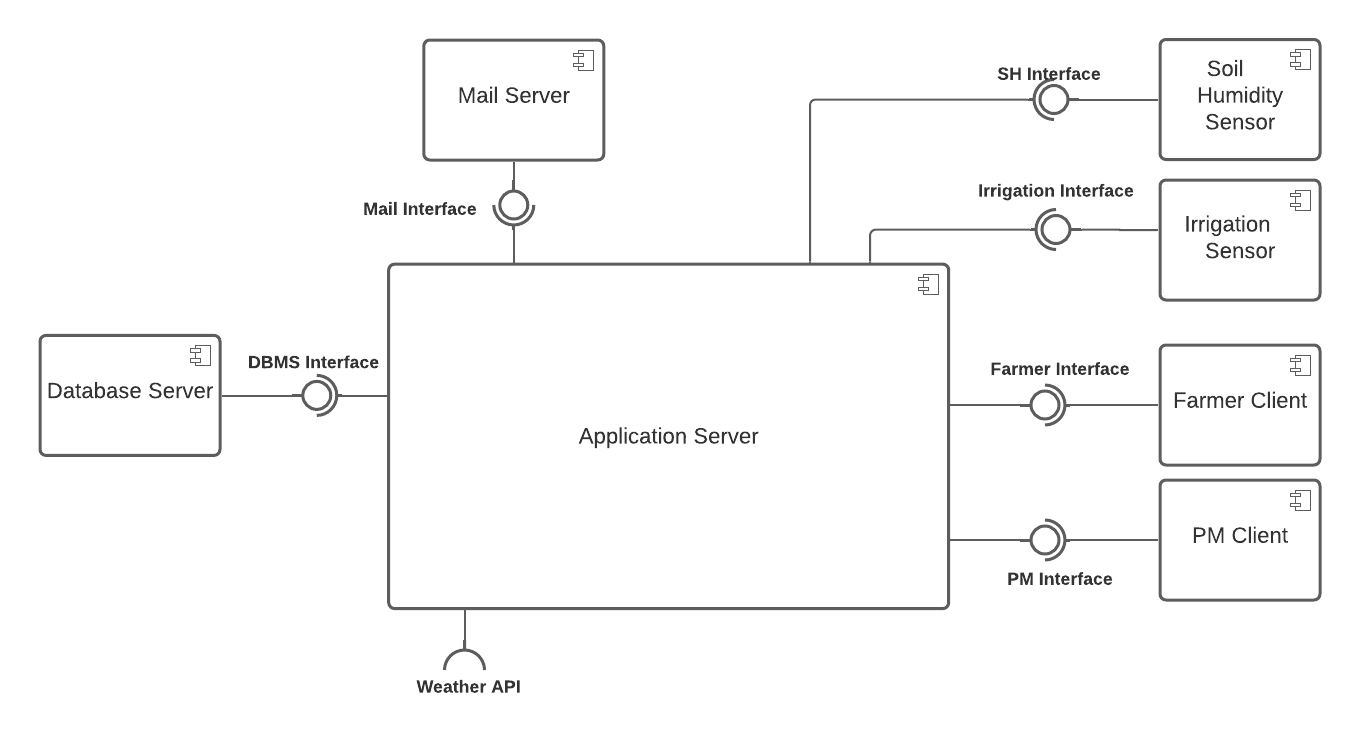
\includegraphics[scale=0.64]{images/hl_component.png}
    \caption{High Level Component Diagram}
    \label{fig:hl_component}
\end{figure}
\subsection{Deployment view}
\subsection{Runtime view}
\subsection{Component Interfaces}
\subsection{Selected Architectural styles and patterns}
\subsection{Other design decisions}

\section{User Interface Desgin}

\section{Requirements Traceability}

\section{Implementation, integration and test plan}

\section{Effort spent}

\bibliography{main.bib}

\end{document}